% Created 2022-06-01 Wed 14:53
% Intended LaTeX compiler: xelatex
\documentclass[letterpaper]{article}
\usepackage{graphicx}
\usepackage{longtable}
\usepackage{wrapfig}
\usepackage{rotating}
\usepackage[normalem]{ulem}
\usepackage{amsmath}
\usepackage{amssymb}
\usepackage{capt-of}
\usepackage{hyperref}
\usepackage[margin=1in]{geometry}
\setlength{\parindent}{0pt}
\usepackage[margin=1in]{geometry}
\usepackage{fontspec}
\usepackage{svg}
\usepackage{tikz}
\usepackage{cancel}
\usepackage{pgfplots}
\usepackage{indentfirst}
\setmainfont[ItalicFont = HelveticaNeue-Italic, BoldFont = HelveticaNeue-Bold, BoldItalicFont = HelveticaNeue-BoldItalic]{HelveticaNeue}
\newfontfamily\NHLight[ItalicFont = HelveticaNeue-LightItalic, BoldFont       = HelveticaNeue-UltraLight, BoldItalicFont = HelveticaNeue-UltraLightItalic]{HelveticaNeue-Light}
\newcommand\textrmlf[1]{{\NHLight#1}}
\newcommand\textitlf[1]{{\NHLight\itshape#1}}
\let\textbflf\textrm
\newcommand\textulf[1]{{\NHLight\bfseries#1}}
\newcommand\textuitlf[1]{{\NHLight\bfseries\itshape#1}}
\usepackage{fancyhdr}
\usepackage{csquotes}
\pagestyle{fancy}
\usepackage{titlesec}
\usepackage{titling}
\makeatletter
\lhead{\textbf{\@title}}
\makeatother
\rhead{\textrmlf{Written} \today}
\lfoot{\theauthor\ \textbullet \ \textbf{2021-2022}}
\cfoot{}
\rfoot{\textrmlf{Page} \thepage}
\renewcommand{\tableofcontents}{}
\titleformat{\section} {\Large} {\textrmlf{\thesection} {|}} {0.3em} {\textbf}
\titleformat{\subsection} {\large} {\textrmlf{\thesubsection} {|}} {0.2em} {\textbf}
\titleformat{\subsubsection} {\large} {\textrmlf{\thesubsubsection} {|}} {0.1em} {\textbf}
\setlength{\parskip}{0.45em}
\renewcommand\maketitle{}
\author{Houjun Liu}
\date{\today}
\title{MVC 2 PS\#31}
\hypersetup{
 pdfauthor={Houjun Liu},
 pdftitle={MVC 2 PS\#31},
 pdfkeywords={},
 pdfsubject={},
 pdfcreator={Emacs 28.0.91 (Org mode 9.5.2)}, 
 pdflang={English}}
\begin{document}

\maketitle
\tableofcontents


\section{Correction factor in Cylindrical}
\label{sec:org65230d6}
For this question, we are actually essentially just doing the Jacobian determinant form for \emph{cylindrical} coordinates.

Turns out, this is actually just saying the same expression for polar, but doing it with an additional, trivial \(z=z\) component.

\begin{equation}
   f(x,y,z) = g(r, \theta,z) 
\end{equation}

Fortunately, this is already derived to use from before.

\begin{equation}
   \begin{cases}
   x = r\cos\theta \\
   y = r\sin\theta \\
   z = z
\end{cases}
\end{equation}

We can then figure out, then the Jacobian determinant. Since the last parameter is \(z=z\), we have:

And therefore, we can figure \(J_{r,\theta,z}\):

\begin{equation}
   J = \begin{bmatrix} 
cos\theta & -r\sin\theta & 0\\
sin\theta & r\cos\theta & 0\\
0 & 0 & 1
\end{bmatrix} 
\end{equation}

The determinant would still, unsurprisingly, be \(r\): you can see this by the fact that each of the "valued" column is multiplied by \(1\), and the last column's determinant is just canceled by \(0\).

Taking its determinant, then:

\begin{equation}
   det(J) = r\cos^2\theta +r\sin^2\theta = r
\end{equation}

And therefore, the change-of-basis result would be:

\begin{equation}
   dx\ dy\ dz = r\ dr\ d\theta\ dz
\end{equation}

\section{Frankenstein coordinates}
\label{sec:org3ca113d}
It seems like Frankenstein coordinates are just the same coordinate system that we are used to, but rotated!

We can actually apply a transformation upon the \((r,\theta)\) choordinates to better describe the system:

\begin{equation}
\begin{cases}
   r = \frac{y}{\cos\phi} \\
   \theta = 90-\phi 
\end{cases}
\end{equation}

\subsection{Draw a point!}
\label{sec:org84734fa}
Draw the point \((\phi = \frac{\pi}{4}, y = 378)\).

\begin{equation}
\begin{cases}
   r = \frac{378}{\frac{\sqrt{2}}{2}} = 378\sqrt{2} \\
   \theta = \frac{\pi}{4}
\end{cases}
\end{equation}

We note that: \(x = r\cos\theta, y=r\sin\theta\), and \(\sin\theta = \cos\theta = \frac{\sqrt{2}}{2}\).

\begin{equation}
\begin{cases}
   x = 378\\
   y = 378
\end{cases}
\end{equation}

\begin{verbatim}
f_dots = points([[378,378]])
plot(f_dots)
\end{verbatim}

\begin{center}
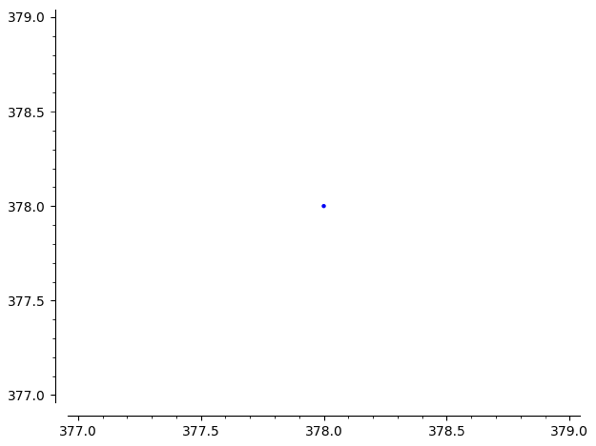
\includegraphics[width=.9\linewidth]{2022-06-01_09-38-21_screenshot.png}
\end{center}

\subsection{Draw another point!}
\label{sec:orgd4a7cc8}
Draw the point \((\phi = \frac{11\pi}{12}, y=-7)\).

\begin{equation}
\begin{cases}
   r = \frac{7}{\frac{1}{4\sqrt{6}} + \frac{1}{4\sqrt{2}}} = \frac{56\sqrt{3}}{\sqrt{2}+\sqrt{6}} \\
   \theta = \frac{-5\pi}{12}
\end{cases}
\end{equation}

We note that: \(x = r\cos\theta, y=r\sin\theta\), \(\sin\theta \approx -0.9659\), \(\cos\theta \approx 0.2588\). Furthermore, we can give \(r=25.1041\). 

Therefore:

\begin{equation}
\begin{cases}
     x = 6.4969\\
    y = -24.2481
\end{cases}
\end{equation}

\begin{verbatim}
f_dots = points([[6.4969, -24.2481]])
plot(f_dots)
\end{verbatim}

\begin{center}
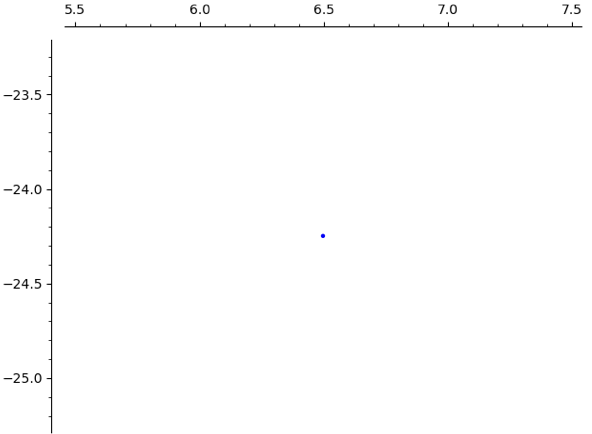
\includegraphics[width=.9\linewidth]{2022-06-01_09-51-33_screenshot.png}
\end{center}

\subsection{A function!}
\label{sec:org8d0b374}
Our nameless function is simply a line at \(y=5\):

\begin{verbatim}
plot(5)
\end{verbatim}

\begin{center}
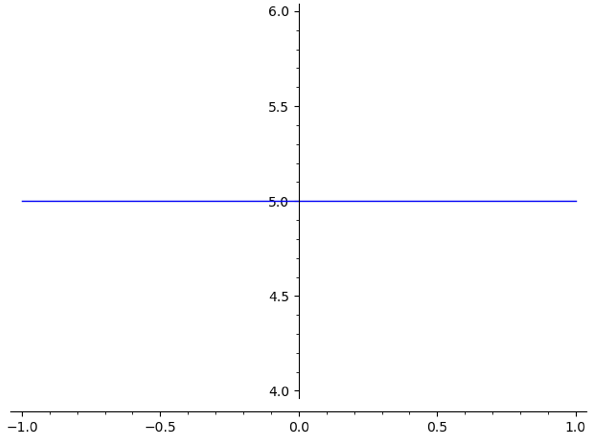
\includegraphics[width=.9\linewidth]{2022-06-01_09-57-14_screenshot.png}
\end{center}

\subsection{Another function.}
\label{sec:orga6492ae}
This function should be more interesting. We are here presented with a shape that increases in its y-dimension radius as the angle increases. Of course, Sage can't actually plot something in our new coordinate frame, so we will convert it to polar to begin:


Recall that---

\begin{equation}
\begin{cases}
   r = \frac{y}{\cos\phi} \\
   \theta = 90-\phi 
\end{cases}
\end{equation}

We therefore convert \((\phi=\phi, y=2\phi)\) to polar:

\begin{equation}
\begin{cases}
r = \frac{2\phi}{\cos\phi}\\
\theta = 90-\phi
\end{cases}
\end{equation}

Manipulating the bottom expression:

\begin{equation}
   \phi = 90-\theta 
\end{equation}

And therefore:

\begin{equation}
   r = \frac{180-2\theta}{sin\theta} 
\end{equation}

\begin{center}
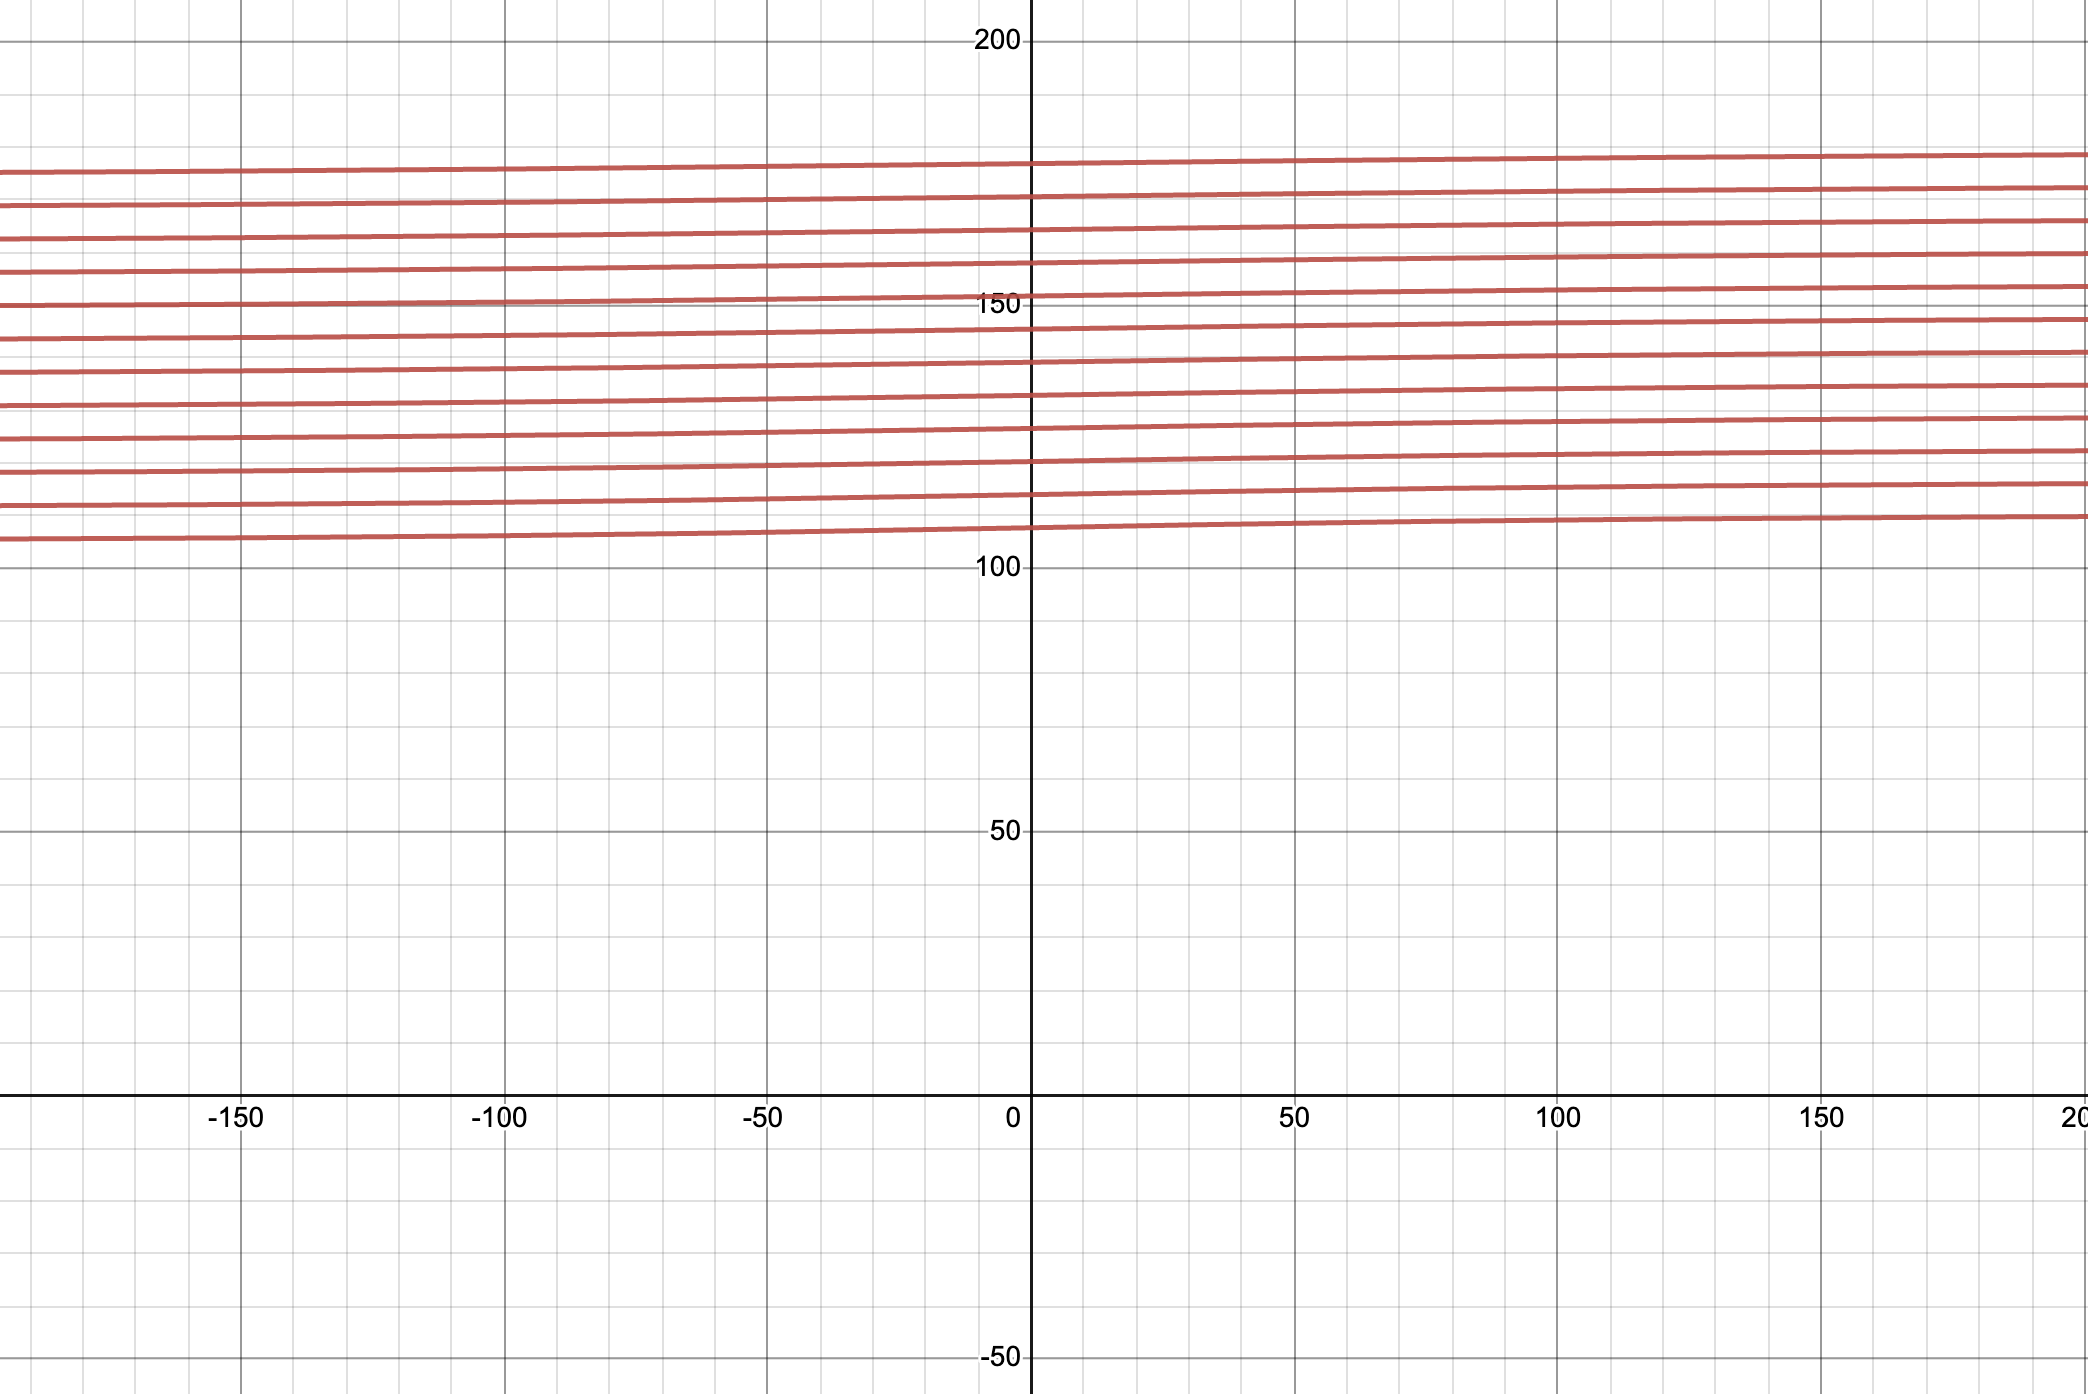
\includegraphics[width=.9\linewidth]{2022-06-01_10-38-51_screenshot.png}
\end{center}

\subsection{First, integral}
\label{sec:orgbcf3b3a}
We can first figure a set of parameterizations for \((x,y)\) for the above choordinates:

Let's figure the \(x\) value. \(x = r\cos\theta = r \sin\phi = \frac{y\sin\phi}{cos\phi} = y\tan\phi\).

\begin{equation}
\begin{cases}
   x = y\tan\phi\\
   y = y 
\end{cases}
\end{equation}

We can take the derivative matrix of this set of parameterizations:

\begin{equation}
   J = \begin{bmatrix} 
\tan\phi & sec^2\phi \\
1 & 0 
\end{bmatrix} 
\end{equation}

Therefore, the correction factor in this case would be \(\sec^2\phi\).

Hence, the integral \(dA = sec^2\phi\ d\phi\ dy\).

\begin{align}
   &\int_5^7 \int_0^{\frac{\pi}{3}} sec^2\phi\ d\phi\ dy\\
& \int_5^7 \sqrt{3} dy\\
& 2\sqrt{3} 
\end{align}

\subsection{Second Integral}
\label{sec:org5e11060}

\begin{align}
   &\int_0^\frac{\pi}{4} \int_0^{\frac{y}{2}} sec^2\phi\ d\phi\ dy\\
& \int_0^\frac{\pi}{4} \tan\frac{y}{2} dy\\
& -2log\left(\frac{\sqrt{\sqrt{2}+2}}{2}\right)
\end{align}

The last step here is computed via Sage.

\section{Parabolic Choordinates}
\label{sec:orga023f23}
Parabolic choordinates are a set of choordinates particularly useful for marginalizing intersecting curved spaces in a parabolic manner. This makes parabolic functions particularly useful to describe.

Its change of bases expressions are:

\begin{equation}
   \begin{cases}
   x = \sigma \tau \\ 
   y = \frac{1}{2}(\tau^2-\sigma^2) 
\end{cases}
\end{equation}

\section{Loxodromic Coordinates}
\label{sec:orga496af8}
Loxodromic Coordinates are choordinates that traverse a spherical surface, crossing the meridians of longitudes at equal angles. This is particularly useful for early navigation, where the sun's angles rendered an important part of the navigation process.

It is a circular path down the shape (take, for instance, the "top-down" projection of the path looks like \(r=\theta\)), yet it winds around a sphere.

The change of bases expressions are:

\begin{equation}
\begin{cases}
x = \cos\lambda \cos\varphi\\
y = \cos\lambda \cos\varphi\\
z = \sin\varphi
\end{cases}
\end{equation}

Where, each point that exhibit intersection with meridian at equal angle is accessible by \(r(\lambda, \varphi)\).
\end{document}